\documentclass[10pt,twocolumn]{article}

\usepackage{iftex}
\ifTUTeX
  \usepackage{fontspec}
\else
  \usepackage[utf8]{inputenc}
  \usepackage[T1]{fontenc}
  \usepackage{lmodern}
\fi
\usepackage[a4paper,margin=1.75cm,columnsep=0.65cm]{geometry}
\usepackage{amsmath,amssymb,amsfonts}
\usepackage{booktabs}
\usepackage{graphicx}
\usepackage{xcolor}
\usepackage{microtype}
\usepackage{enumitem}
\usepackage[font=small,labelfont=bf]{caption}
\usepackage[colorlinks=true,linkcolor=blue!70!black,citecolor=blue!70!black,urlcolor=blue!70!black]{hyperref}

\setlength{\parskip}{2.5pt}
\setlength{\parindent}{1em}
\setlength{\emergencystretch}{1.4em}
\setlist[itemize]{leftmargin=1.4em,itemsep=1.5pt,topsep=2pt}
\setlist[enumerate]{leftmargin=1.5em,itemsep=1.5pt,topsep=2pt}

\title{\Large\bfseries Self-Indexed Sparse SwiGLU: Zero-Training Coarse-to-Fine Routing,\\Negative-Overhead Mixed-Precision Storage, and Pre-Attention PCIe~5.0 Prefetching}

\author{
  \textbf{Ferenc Frész}\\
  \href{mailto:ferenc.fresz@gmail.com}{\texttt{ferenc.fresz@gmail.com}} $\cdot$ \href{https://github.com/ferencfresz/ffmod01}{\texttt{github.com/ferencfresz/ffmod01}}
}
\date{November 2026}

\begin{document}
\maketitle

\begin{abstract}
Autoregressive Large Language Model (LLM) decoding at low batch sizes is fundamentally bottlenecked by memory bandwidth, with Feed-Forward Networks (FFNs) accounting for $85\text{--}90\%$ of parameter traffic in Grouped-Query Attention (GQA) Transformers. Prior sparse inference engines face a sharp trilemma: learned-predictor runtimes (\emph{DejaVu}, \emph{PowerInfer}) require ReLU conversion and auxiliary predictor training that inflates VRAM; gate-thresholding methods (\emph{CATS}) still read $100\%$ of the dense gate matrix; and coordinate-pruning methods (\emph{TEAL}) corrupt exact inner products past $40\text{--}50\%$ sparsity.

We introduce \textbf{FFMod}, a zero-training, zero-calibration inference architecture built on the principle of separating \emph{knowledge storage} from \emph{dynamic compute planning}. First, FFMod constructs a self-indexed dual-branch \textbf{Smooth-INT4 $\times$ Top-$D$} router directly from any pretrained SwiGLU or GeGLU weight triplet, estimating true channel impact $|\mathrm{SiLU}(\hat{g}_i)\hat{u}_i|\cdot\|W_{\mathrm{down}}[:,i]\|_2$ using $<5\%$ of dense memory traffic while evaluating winning channels in full hidden dimension $H$. Second, we propose \textbf{BitSplit-12} (per-channel \texttt{FP8} gate/up paired with \texttt{BF16} down projections), eliminating the index memory tax to reduce total model VRAM by $13.0\%$ (\texttt{BitSplit-12}) to $26.1\%$ (full \texttt{FP8}) while outperforming dense \texttt{cuBLAS} Tensor Cores by up to $2.55\times\text{--}3.54\times$ per FFN layer ($1.57\times\text{--}1.70\times$ end-to-end token throughput on an NVIDIA RTX~5090 Blackwell GPU, including $1.51\times$ at speculative micro-batch $N=4$). Third, we uncover the \emph{KV-Cache Pollution Paradox} and introduce a KV-safe hybrid layer sparsity schedule alongside a \textbf{12-SM Open-Page DDR5 UVA} tiered offloading engine over PCIe~5.0. By prefetching a high-confidence core subset prior to Self-Attention and overlapping exact post-attention delta verification inside a two-stream fork-join \texttt{CUDAGraph}, FFMod achieves $96\text{--}99\%$ compute/DMA overlap and enables heavyweight 32B+ SwiGLU models ($65.5$~GB \texttt{BF16}) to run interactively inside $16\text{--}22$~GB consumer VRAM budgets.
\end{abstract}

\section{Introduction}
Modern open-weight LLMs---including Llama-3, Qwen2.5~\cite{qwen25_2024}, Mistral, DeepSeek, and Gemma-2---universally combine Grouped-Query Attention (GQA)~\cite{ainslie2023gqa} with gated MLP blocks (SwiGLU or GeGLU)~\cite{shazeer2020glu}. While GQA shrinks attention weights and KV-cache footprints by $4\times\text{--}8\times$, the SwiGLU FFN expands to three wide matrices ($W_{\mathrm{gate}}, W_{\mathrm{up}} \in \mathbb{R}^{I\times H}$ and $W_{\mathrm{down}} \in \mathbb{R}^{H\times I}$). In \texttt{Qwen2.5-3B} ($H=2048, I=11008$), FFN matrices represent $87.7\%$ of transformer-block parameters ($4.87$~GB streamed per generated token); in \texttt{Qwen2.5-32B} ($H=5120, I=27648$, $64$~layers), they represent $54.36$~GB out of $65.5$~GB in \texttt{BF16}. During single-request or small-batch ($N\in[1,8]$) decoding, arithmetic intensity is $O(N)$ FLOPs/byte, leaving GPU Tensor Cores starved behind GDDR7 or PCIe memory transfers.

Conventional engines conflate \emph{how parameters are stored} with \emph{how they are accessed}, executing dense matrix-vector multiplications across all $I$ intermediate channels on every token. Existing attempts to break this dense paradigm suffer from three structural limitations:
\begin{enumerate}
  \item \textbf{ReLU-fication \& Predictor Overhead:} Systems such as DejaVu~\cite{liu2023dejavu} and PowerInfer~\cite{song2024powerinfer} rely on trained MLP predictors and exact ReLU zeros~\cite{mirzadeh2024relustrikesback}. Native SwiGLU models lack hard zeros and exhibit high-rank mid-tier channel activations that defeat low-rank ($r=64$) linear routers while inflating VRAM by $15\text{--}25\%$.
  \item \textbf{Partial Projection Reads or Inexact Inner Products:} Training-free methods like CATS~\cite{lee2024cats} compute $100\%$ of $W_{\mathrm{gate}} x$ in full precision (reading a mandatory $33.3\%$ floor of FFN weights) and require calibration thresholds. Input-pruning methods like TEAL~\cite{liu2025teal} and rank approximations like R-Sparse~\cite{zhang2025rsparse} truncate coordinates inside the final computation itself, causing sharp KL divergence growth beyond $45\text{--}50\%$ sparsity.
  \item \textbf{Reactive vs.\ Lossy PCIe Offloading:} When model weights exceed GPU VRAM, reactive fetching stalls the GPU behind PCIe latency, whereas purely speculative pre-attention routing drops attention-induced ``surprise'' channels.
\end{enumerate}

\textbf{Contributions.} We present \textbf{FFMod}, an end-to-end sparse SwiGLU/GeGLU runtime that resolves all three limitations without retraining or calibration data:
\begin{itemize}
  \item \textbf{Empirical Characterization \& KV-Cache Paradox (\S\ref{sec:empirical}):} Across seven controlled studies, we show that $G=1$ transposed channels ($3H$ bytes $= 12\text{--}15$~KB) naturally saturate 128-byte GPU cache lines, top-$2\%$ dynamic outlier spikes carry $65.2\%$ of $L_2^2$ FFN energy, and aggressive early-layer sparsity degrades downstream tokens via \emph{KV-cache error compounding}.
  \item \textbf{Self-Indexed Smooth-INT4 $\times$ Top-$D$ Router (\S\ref{sec:router}):} Borrowing asymmetric quantization principles from vector search~\cite{guo2020scann,gao2024rabitq}, we pack smoothed 4-bit representations of both $W_{\mathrm{gate}}$ and $W_{\mathrm{up}}$ into a coalesced 32-bit strided-4 layout scanned over only the top-$D$ weighted input coordinates ($\sim 4.7\%$ traffic), followed by exact full-$H$ evaluation of the winning $K=(1-s)I$ channels in custom Triton~\cite{tillet2019triton} kernels.
  \item \textbf{Asymmetric \texttt{BitSplit-12} \& \texttt{FP8} Kernels (\S\ref{sec:bitsplit}):} Exploiting the asymmetric noise sensitivity of $\mathrm{SiLU}(g)\odot u$ versus $W_{\mathrm{down}}$, \texttt{BitSplit-12} stores gate/up channels in \texttt{FP8} and down channels in \texttt{BF16}, cutting total VRAM by $13.0\%$ ($5.37$~GB vs.\ $6.17$~GB dense) while delivering $2.36\times$ FFN speedup at $N=1$ and $1.51\times$ over \texttt{cuBLAS} Tensor Cores at speculative $N=4$.
  \item \textbf{PCIe~5.0 Open-Page DDR5 Tiered Engine (\S\ref{sec:tiered}):} We identify severe DDR5 row-buffer bank thrashing when all GPU SMs issue concurrent UVA gathers, boosting PCIe~5.0 random channel gather bandwidth by $+22\text{--}29\%$ ($37.7\text{--}38.5$~GB/s) using a 12-SM coalesced \texttt{int64} gather kernel that leaves $85\%$ of GPU SMs free ($96\text{--}99\%$ overlap). Paired with \emph{High-Confidence Core Prefetch + Exact Post-Attention Delta Fixup} inside a two-stream \texttt{CUDAGraph}, FFMod runs \texttt{Qwen2.5-32B-Instruct} cleanly within $16\text{--}22$~GB VRAM.
\end{itemize}

\section{Empirical Motivation \& Oracle Analysis}
\label{sec:empirical}

Consider a SwiGLU FFN layer mapping hidden state $x \in \mathbb{R}^H$ to output $y \in \mathbb{R}^H$ across $I$ channels:
\begin{equation}
  \begin{aligned}
    y(x) &= \sum_{i=1}^{I} z_i(x)\, w_{\mathrm{down},:,i}, \\
    z_i(x) &= \mathrm{SiLU}(w_{\mathrm{gate},i}^\top x)\cdot (w_{\mathrm{up},i}^\top x).
  \end{aligned}
  \label{eq:swiglu}
\end{equation}
The true Euclidean contribution of channel $i$ to $y(x)$ is precisely $\|z_i(x)\,w_{\mathrm{down},:,i}\|_2 = |z_i(x)|\cdot\|w_{\mathrm{down},:,i}\|_2$. Note that ordering channels solely by $|w_{\mathrm{gate},i}^\top x|$ (as in CATS~\cite{lee2024cats}) ignores both the multiplicative $w_{\mathrm{up},i}^\top x$ branch and column norms $\|w_{\mathrm{down},:,i}\|_2$.

\begin{figure*}[t]
  \centering
  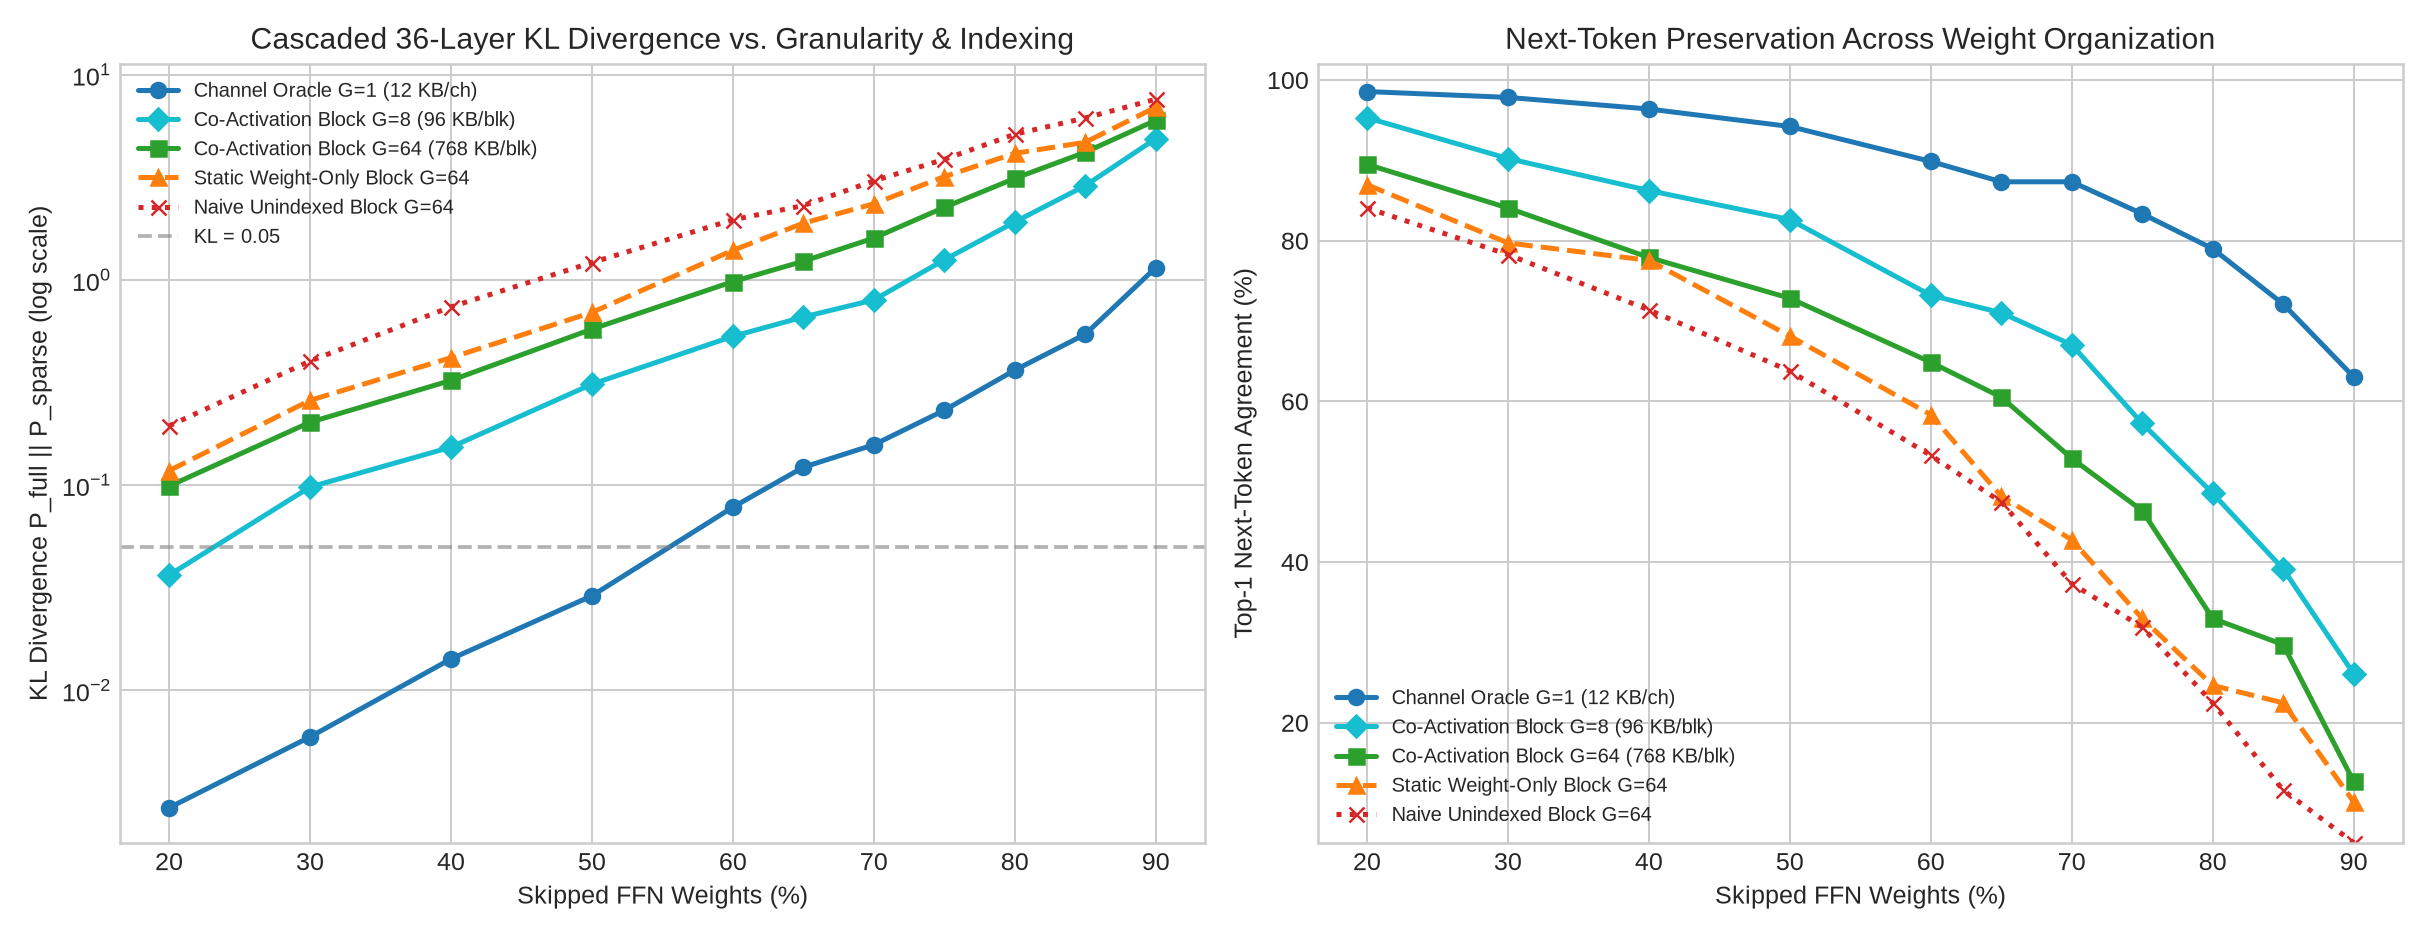
\includegraphics[width=0.95\textwidth]{../results/plots/fig1_oracle_and_indexing.png}
  \caption{\textbf{Experiment 1:} Cascaded 36-layer Oracle FFN sparsity on \texttt{Qwen2.5-3B} across held-out domains. Channel granularity ($G=1$, $12$~KB/channel) dramatically outperforms coarse block grouping ($G=8,64$), while zero-data cosine weight permutation cuts $G=64$ KL error by $43\%$.}
  \label{fig:exp1}
\end{figure*}

\subsection{Granularity $G=1$ vs.\ Block Permutation}
Because Eq.~\eqref{eq:swiglu} is permutation-invariant over $i \in \{1,\dots,I\}$, we first evaluate cascaded 36-layer Oracle pruning across channel granularities $G \in \{1, 8, 64\}$ on held-out English factual, mathematical reasoning, Python coding, and morphologically rich Hungarian prompts (Fig.~\ref{fig:exp1}). While balanced cosine clustering of static $W_{\mathrm{gate}}$ rows reduces $G=64$ KL divergence by $43\%$ with zero calibration data ($1.214 \to 0.694$ at $50\%$ skip), individual channel selection ($G=1$) achieves $42\times$ lower KL divergence ($\mathrm{KL}=0.0289$, $94.2\%$ Top-1 match at $50\%$ skip; $\mathrm{KL}=0.1572$, $87.3\%$ Top-1 at $70\%$ skip). Crucially, when storing $[w_{\mathrm{gate},i}; w_{\mathrm{up},i}; w_{\mathrm{down},:,i}^\top]$ contiguously as $[I, 3, H]$, a single $G=1$ channel spans $3H$ elements ($12$~KB in \texttt{BF16} at $H=2048$; $15$~KB in \texttt{FP8} at $H=5120$), comprising $96\text{--}120$ full 128-byte GPU cache lines---eliminating any hardware need for $G=64$ grouping. Conversely, skipping even $8/36$ whole FFN layers collapses accuracy to $55.1\%$ Top-1 ($\mathrm{KL}=1.84$).

\begin{figure}[t]
  \centering
  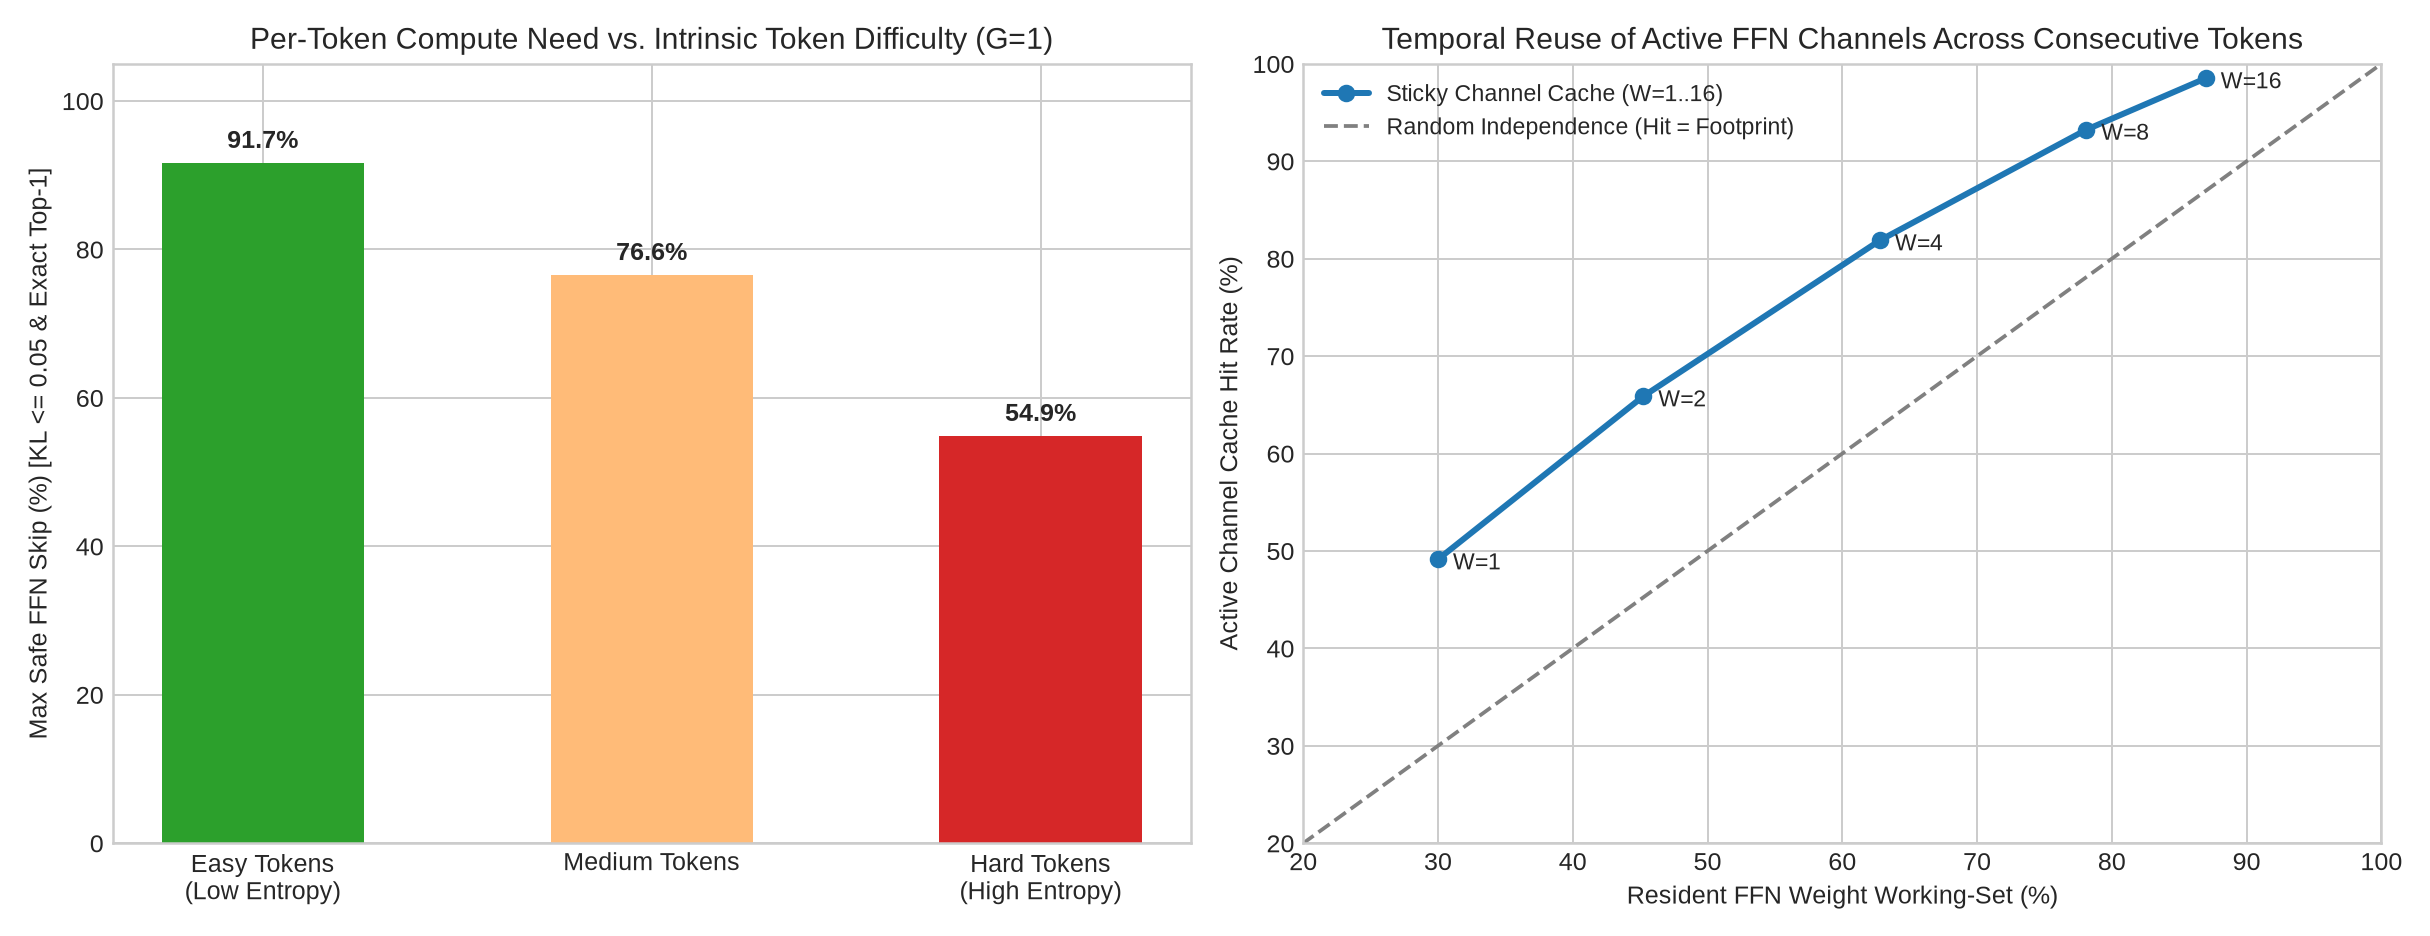
\includegraphics[width=\columnwidth]{../results/plots/fig2_difficulty_and_temporal.png}
  \caption{\textbf{Experiments 1--2:} Token-wise maximum safe FFN skip ratio $s^*(t)$ correlates strongly with output entropy ($\rho = -0.855$, $p < 10^{-70}$), while a 4-token sliding sticky channel cache captures $81.9\%$ of active channels.}
  \label{fig:exp2}
\end{figure}

\subsection{Outlier Energy, Temporal Locality \& Rank Bottleneck}
Analyzing per-token difficulty (Fig.~\ref{fig:exp2}), the maximum sparsity preserving Top-1 identity and $\mathrm{KL}\le 0.05$ averages $74.4\%$ ($91.7\%$ on low-entropy syntax tokens vs.\ $54.9\%$ on high-entropy reasoning steps; Spearman $\rho=-0.855$). Consecutive tokens share $49.1\%$ of active channels ($60.3\%$ in layers $0\text{--}11$), giving an $81.9\%$ hit rate under a $W=4$ sticky cache.

Furthermore, decomposing $L_2^2$ FFN output energy reveals extreme heavy-tailed concentration: the \textbf{top $2\%$ of channels ($220/11008$) generate $65.2\%$ of total FFN energy}, and $88.6\%$ of these are rare dynamic spikes firing on $<20\%$ of tokens. Zero-GEMM cross-layer Markov transition tables ($\ell-1 \to \ell$) achieve a $12.4\times$ recall lift on these spikes. Yet a calibrated rank-$64$ neural MLP router (\S\ref{sec:router}, Fig.~\ref{fig:exp3}) plateaus at $64.5\%$ overall channel recall ($\mathrm{KL}=0.450$ at $50\%$ skip): while rank-$64$ captures $89\%$ of top-$1\%$ spikes, the remaining $35\%$ energy resides in mid-tier channels ($2\%\text{--}35\%$) whose inner products span full rank $H=2048$ and blur through any low-rank linear bottleneck.

\begin{figure}[t]
  \centering
  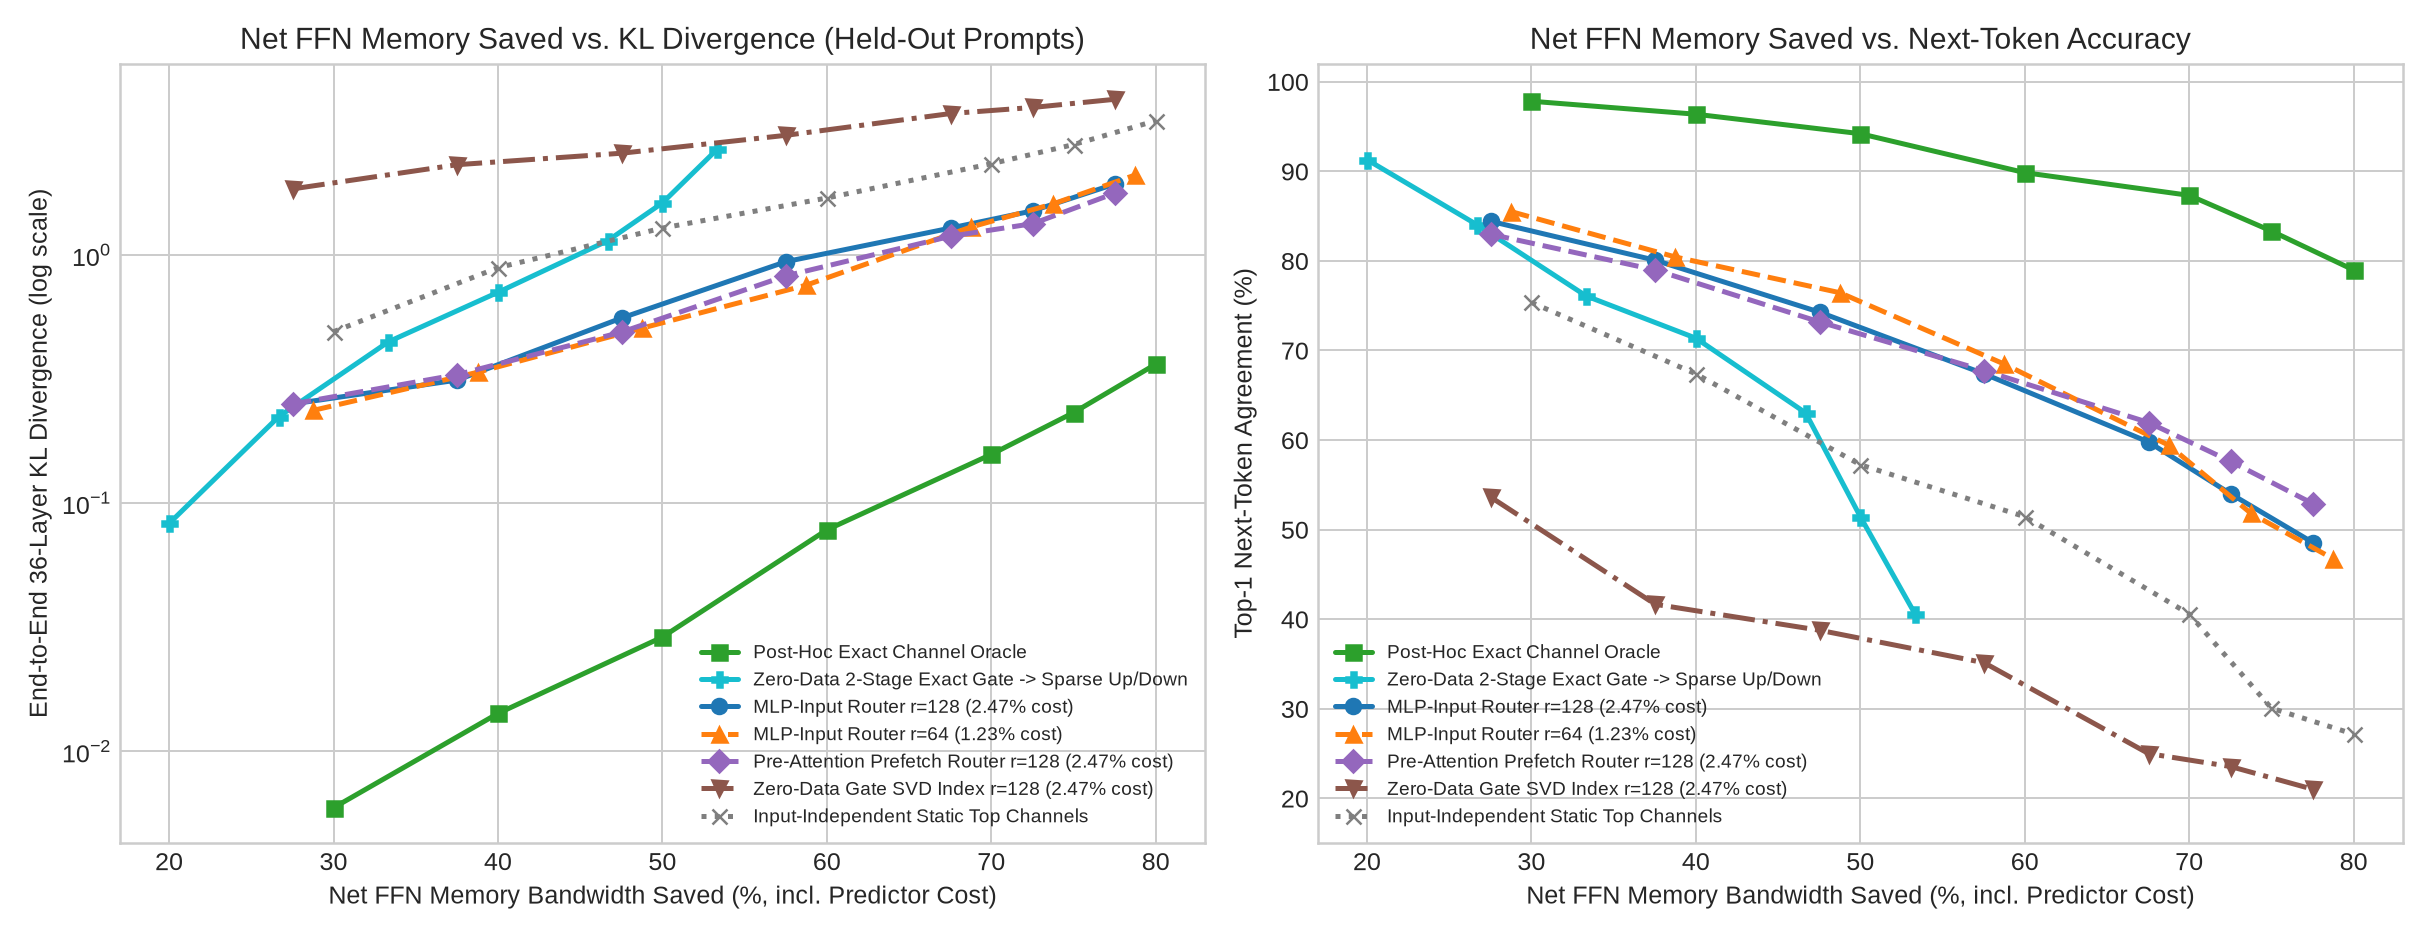
\includegraphics[width=\columnwidth]{../results/plots/fig3_ahead_of_time_predictors.png}
  \caption{\textbf{Experiment 3:} Low-rank ($r=64$) predictors confirm that pre-attention hidden states already predict post-attention FFN channels, but suffer a linear rank bottleneck against full-rank mid-tier channels.}
  \label{fig:exp3}
\end{figure}

\subsection{The KV-Cache Pollution Paradox}
\label{sec:kvparadox}
In Experiment~5 (Fig.~\ref{fig:exp4}), we first derive a zero-FLOP affine bias/gain correction for asymmetric SiLU truncation ($\bar{z}_\ell = \mathbb{E}[z_\ell(x)] \neq 0$), cutting KL error of low-rank routers by $21\text{--}29\%$. Next, we train a lightweight probe at layer~6 that predicts final layer-36 token entropy ($\rho=0.653, p=6.6\times 10^{-35}$) to dynamically skip $85\text{--}90\%$ of FFN channels on ``easy'' tokens.

Surprisingly, while dynamic token-difficulty routing improves single-step accuracy on prose, it increases multi-token KL error on code ($0.186 \to 0.506$). Tracing \texttt{def quicksort} exposes a fundamental autoregressive phenomenon we term the \textbf{KV-Cache Pollution Paradox}: when processing \texttt{" quick"}, predicting \texttt{"sort"} has near-zero entropy ($H=2.5\times 10^{-4}$). Pruning $90\%$ of layers $6\text{--}35$ still emits \texttt{"sort"} correctly at step $t$, \emph{but permanently writes degraded Key/Value projections for \texttt{" quick"} into the KV cache of layers $7\text{--}35$}. Twenty tokens later, when the recursive call \texttt{return quicksort(left)} attends back to \texttt{" quick"}, attention reads corrupted KV states. Consequently, aggressive sparsity must either preserve directional fidelity uniformly or restrict high skip ratios ($75\text{--}80\%$) to the upper third of layers ($\ell \ge \lfloor 2L/3\rfloor$), after core semantic KV states have stabilized.

\begin{figure}[t]
  \centering
  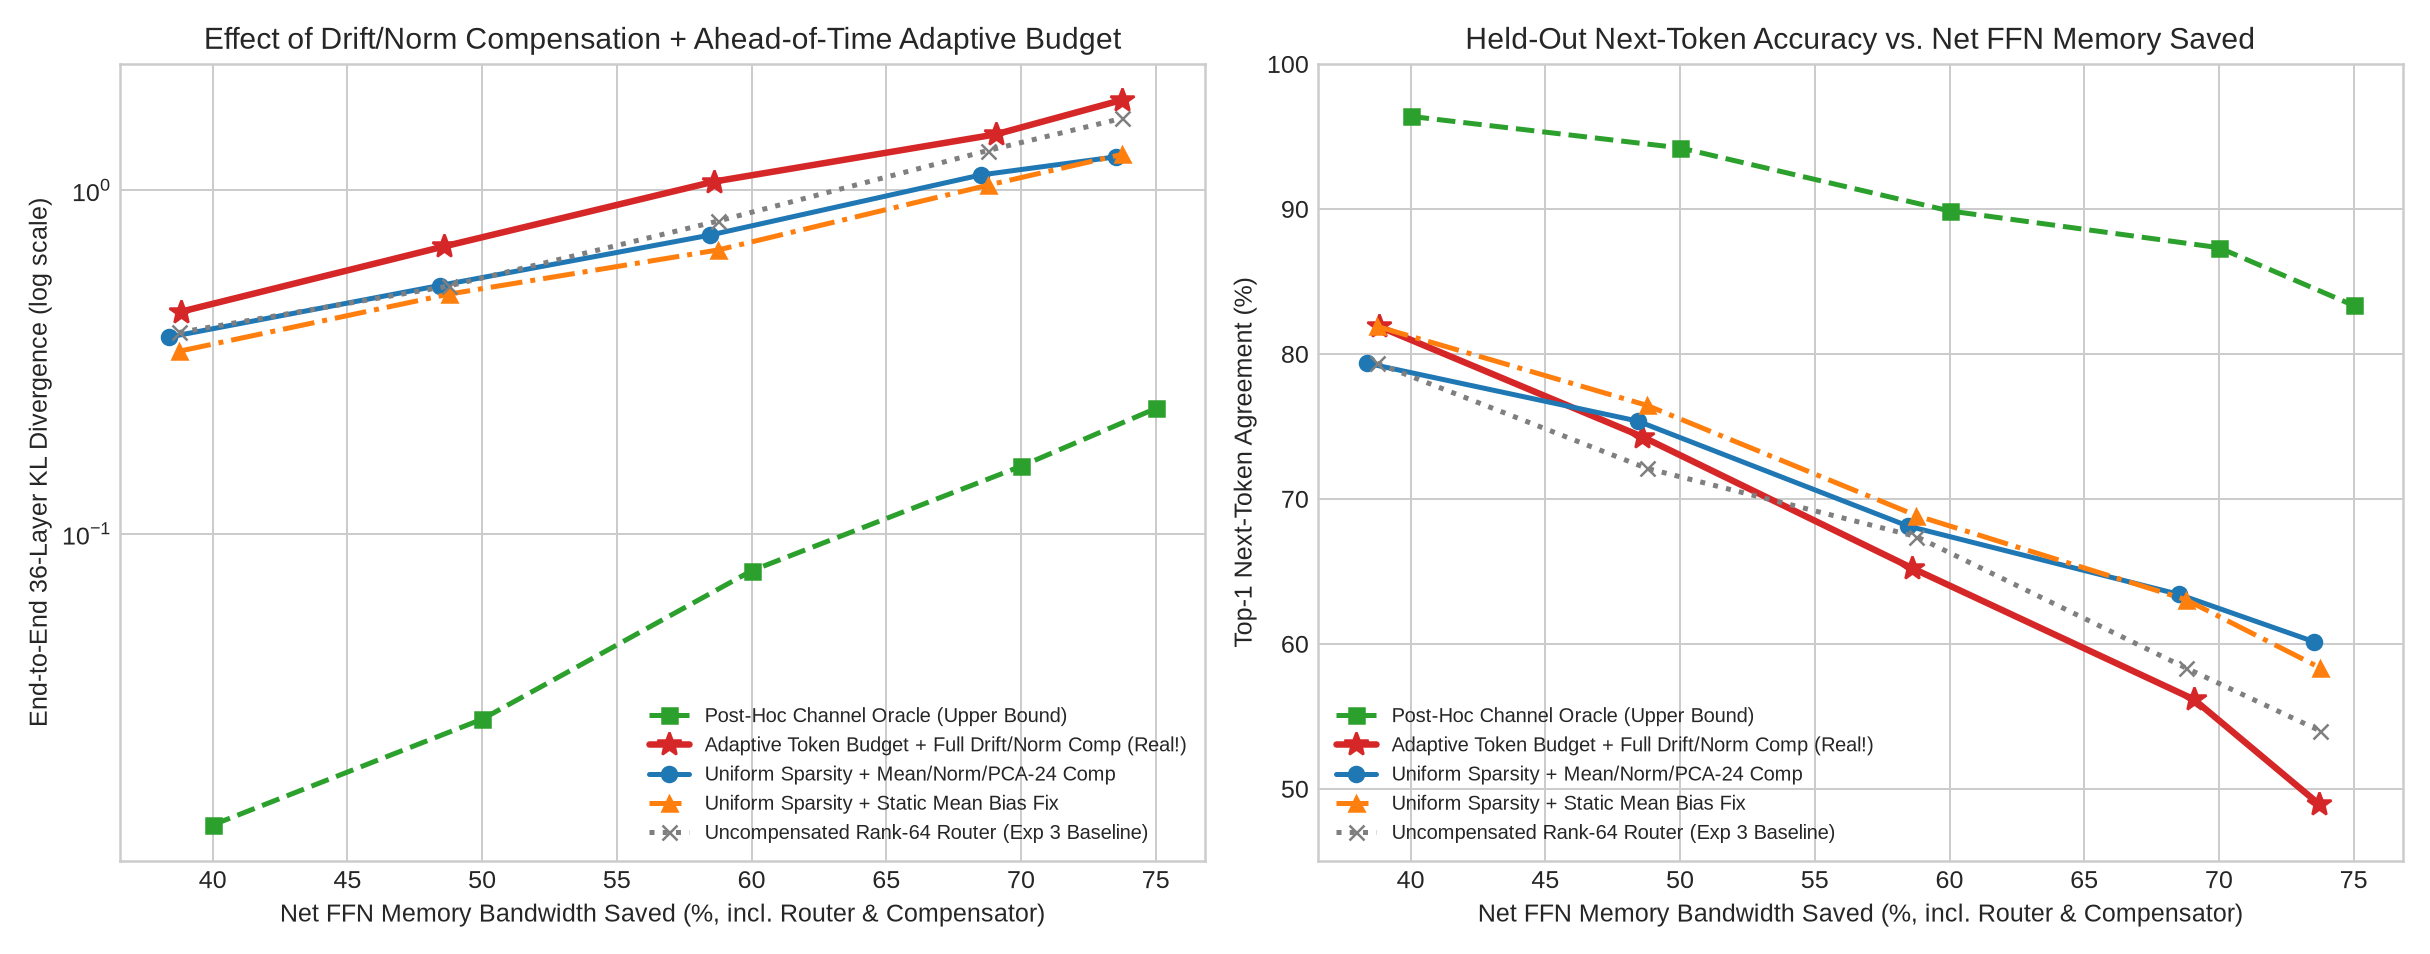
\includegraphics[width=\columnwidth]{../results/plots/fig4_compensated_adaptive_engine.png}
  \caption{\textbf{Experiment 5:} Static SiLU bias/gain compensation and empirical demonstration of the KV-Cache Pollution Paradox under early-layer aggressive token pruning.}
  \label{fig:exp4}
\end{figure}

\section{Zero-Data Coarse-to-Fine Weight Indexing}
\label{sec:router}

To eliminate both training/calibration dependencies and low-rank bottlenecks, FFMod treats static FFN weight matrices as an \emph{indexable database} queried by hidden state $x$.

\subsection{Smooth-INT4 $\times$ Top-$D$ Asymmetric Formulation}
Activation outliers in $x$ otherwise dominate naive quantization of $W_{\mathrm{gate}}$ and $W_{\mathrm{up}}$. Inspired by SmoothQuant~\cite{xiao2023smoothquant}---but computed \emph{strictly from static weights with zero calibration tokens}---we define per-coordinate smoothing factors ($\alpha=0.5$):
\begin{equation}
  c_{g,j} = \left(\frac{1}{I}\sum_{i=1}^I W_{\mathrm{gate},i,j}^2\right)^{\!\!1/4}\!\!, \quad
  c_{u,j} = \left(\frac{1}{I}\sum_{i=1}^I W_{\mathrm{up},i,j}^2\right)^{\!\!1/4}\!\!.
\end{equation}
Dividing columns by $c_{g,j}, c_{u,j}$ and applying MSE-optimal Gaussian clipping ($2.9\,\mathrm{RMS}/7.5$), each normalized row is quantized to unsigned 4-bit integers $Q_{g,i,j}, Q_{u,i,j} \in \{0,\dots,15\}$ with row scales $r_{g,i}, r_{u,i}$:
\begin{equation}
  \begin{aligned}
    W_{\mathrm{gate},i,j} &\approx r_{g,i}\,(Q_{g,i,j} - 7.5)\,c_{g,j}, \\
    W_{\mathrm{up},i,j} &\approx r_{u,i}\,(Q_{u,i,j} - 7.5)\,c_{u,j}.
  \end{aligned}
\end{equation}
At runtime, Stage~1 scales input coordinates $\tilde{x}_{g,j} = x_j c_{g,j}$, $\tilde{x}_{u,j} = x_j c_{u,j}$ and selects only the \textbf{top-$D$ coordinates} $\mathcal{D}(x) \subset \{1,\dots,H\}$ maximizing $|x_j|\sqrt{c_{g,j}^2 + c_{u,j}^2}$ (typically $D/H \in [0.25, 0.375]$). Scanning only $j \in \mathcal{D}(x)$ yields full-rank estimates $\hat{g}_i, \hat{u}_i$ for all $I$ channels, scored by exact $L_2$ impact:
\begin{equation}
  \hat{s}_i(x) = \big|\phi(r_{g,i}\hat{g}_i)\cdot \hat{u}_i\big|\cdot \big(r_{u,i}\|W_{\mathrm{down},:,i}\|_2\big),
  \label{eq:score}
\end{equation}
where $\phi$ is $\mathrm{SiLU}$ or $\mathrm{GELU}_{\tanh}$. Reading $D$ rows of two 4-bit matrices transfers $D \cdot I$ bytes---just $4.17\%$ ($D=512$) to $6.25\%$ ($D=768$) of the $6HI$-byte dense \texttt{BF16} FFN! As shown in Fig.~\ref{fig:exp5}, this zero-data index lifts $50\%$-skip Top-1 agreement from $78.6\%$ (calibrated MLP router) to \textbf{$92.8\%$} ($\mathrm{KL}=0.1039$), nearly matching the hindsight Oracle ($94.2\%$).

\begin{figure*}[t]
  \centering
  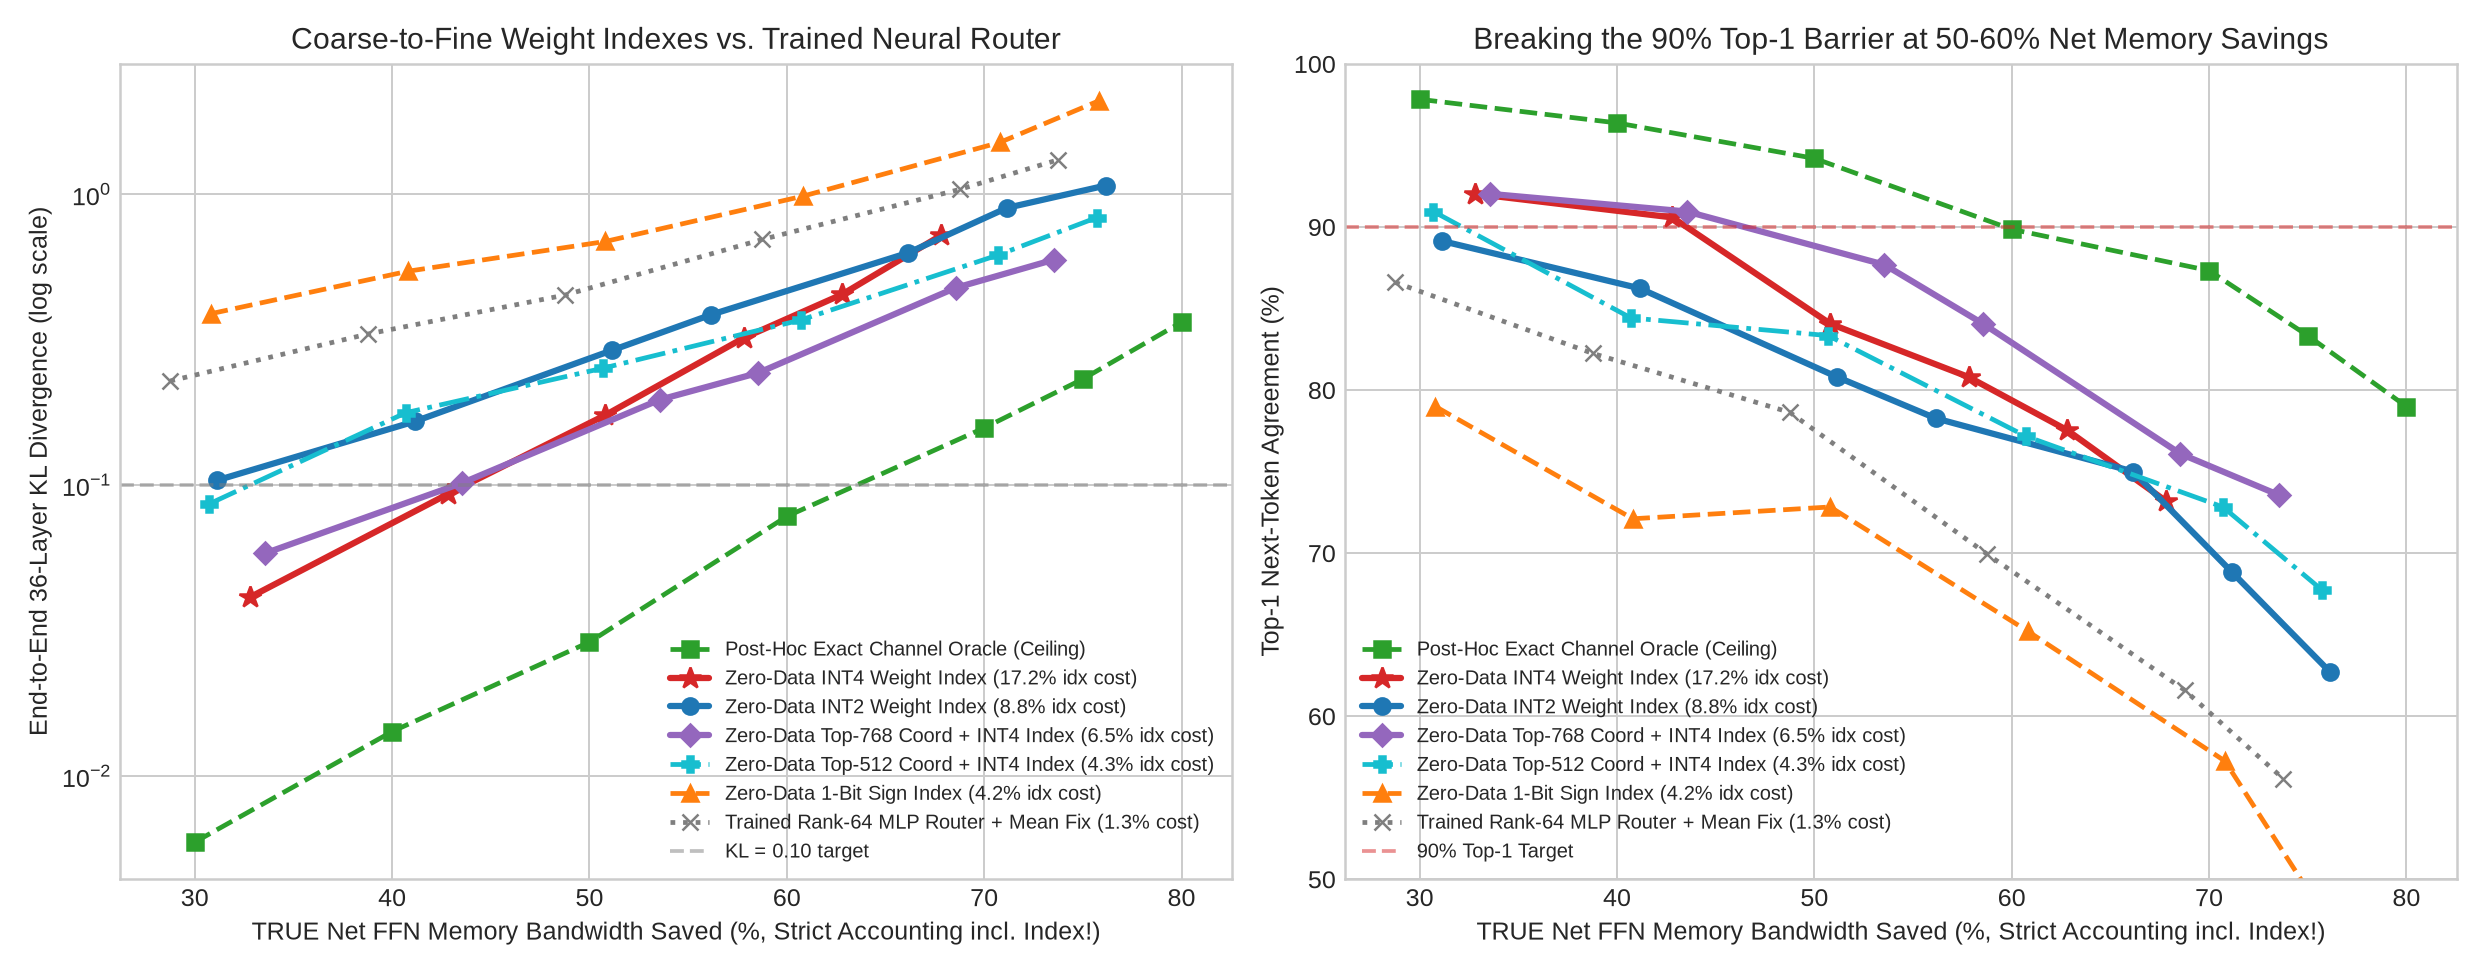
\includegraphics[width=0.95\textwidth]{../results/plots/fig5_coarse_to_fine_routers.png}
  \caption{\textbf{Experiment 6:} Zero-data coarse-to-fine weight indexes (\texttt{RaBitQ} 1-bit and \texttt{Top-D + Smooth-INT4}) decisively outperform calibrated rank-64 neural routers across recall, KL divergence, and Top-1 agreement.}
  \label{fig:exp5}
\end{figure*}

\subsection{Four-Stage Synchronization-Free Triton Pipeline}
Random gather overhead can easily negate theoretical FLOP savings on modern GPUs. We engineer a synchronization-free, 100\% \texttt{CUDAGraph}-capturable four-kernel Triton~\cite{tillet2019triton} pipeline whose intermediate buffers ($\le 352$~KB) remain strictly inside the 64~MB L2 cache:
\begin{enumerate}
  \item \textbf{\texttt{k1\_prologue} ($\sim 7.9\,\mu$s):} Computes $\tilde{x}_g, \tilde{x}_u$, zeros the FP32 accumulator, and extracts top-$D$ indices via 18-step \emph{$\log_2$-domain register binary search} ($0.03\%$ threshold precision across 40 orders of magnitude, immune to attention-sink outliers) compacted with \texttt{tl.cumsum}.
  \item \textbf{\texttt{k2\_2d\_splitd\_int4\_scan} ($10.7\text{--}14.3\,\mu$s, $\sim 600$~GB/s):} Packs 4 channels of $(Q_g, Q_u)$ nibbles per 32-bit \texttt{int32} word in a \emph{strided-4} $[H, I/4]$ layout (zero inner-loop scale loads). By tiling across both channel blocks (\texttt{BLOCK\_I4=128}) and coordinate splits (\texttt{SPLIT\_D=8, TILE\_D=8}), 176 CTAs issue 8 concurrent vectorized indirect row loads per loop step---Satisfying Little's Law to cut latency by \textbf{$5.8\times$} ($82.6\,\mu\text{s} \to 14.3\,\mu\text{s}$).
  \item \textbf{\texttt{k3\_reduce\_select} ($\sim 13.0\,\mu$s):} Reduces L2-resident partial sums, evaluates Eq.~\eqref{eq:score} (taking the element-wise maximum across micro-batches $N \in [1,8]$ for union-active speculative verification), and selects $K=(1-s)I$ sorted channel indices.
  \item \textbf{\texttt{k4\_fused\_sparse\_epilogue} ($61.6\,\mu$s at $65\%$ skip, $781$~GB/s):} Prefetches $[w_{\mathrm{gate},i}, w_{\mathrm{up},i}, w_{\mathrm{down},:,i}^\top]$ simultaneously \emph{before} warp-level \texttt{tl.sum} synchronization, accumulates into register tiles (up to \texttt{BLOCK\_H=8192}), and converts FP32 to BF16 via an atomic last-CTA epilogue without an extra kernel launch.
\end{enumerate}

\begin{figure*}[t]
  \centering
  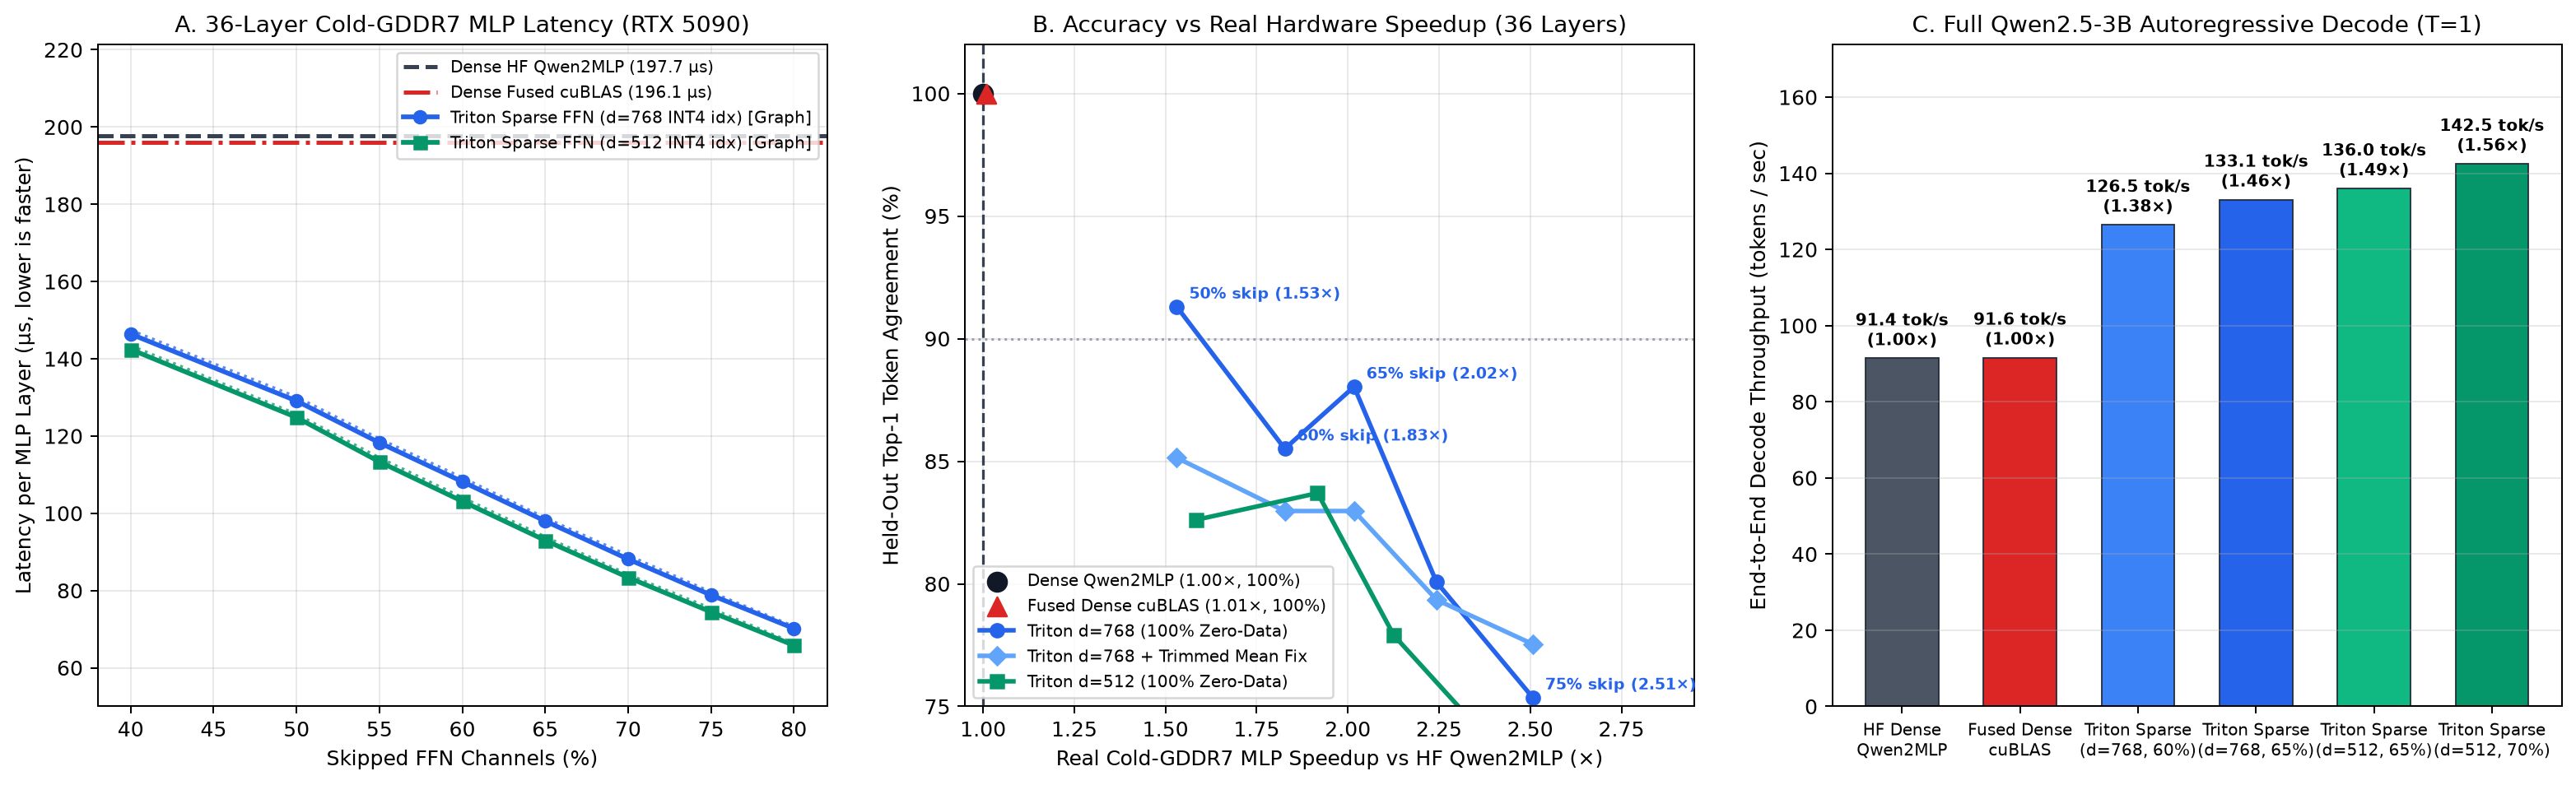
\includegraphics[width=0.97\textwidth]{../results/plots/fig6_triton_wallclock_speedup.png}
  \caption{\textbf{Experiment 7:} Real cold-GDDR7 36-layer wall-clock latency and full-model \texttt{Qwen2.5-3B} generation speedup on RTX~5090 against 3-GEMV \texttt{Qwen2MLP} and 2-GEMV \texttt{FusedCuBLAS} baselines.}
  \label{fig:exp6}
\end{figure*}

\section{Negative-Overhead Mixed-Precision Storage (\texttt{BitSplit-12} \& \texttt{FP8})}
\label{sec:bitsplit}

Storing a \texttt{Smooth-INT4} index alongside \texttt{BF16} weights adds $+13.2\%$ VRAM ($6.99$~GB vs.\ $6.17$~GB on \texttt{Qwen2.5-3B}). To achieve \emph{zero} (in fact, negative) memory overhead while accelerating Stage~2 further, we exploit the structural asymmetry of SwiGLU: quantization noise in $w_{\mathrm{gate},i}^\top x$ and $w_{\mathrm{up},i}^\top x$ is damped on inactive gates by $\mathrm{SiLU}(\cdot)$, whereas $w_{\mathrm{down},:,i}$ adds directly onto the residual stream.

We introduce \textbf{BitSplit-12}, storing $[w_{\mathrm{gate},i}, w_{\mathrm{up},i}]$ in per-channel \texttt{float8\_e4m3fn} ($2H$ bytes) and $w_{\mathrm{down},:,i}$ in \texttt{bfloat16} ($2H$ bytes). Combined with the $1$-byte/channel \texttt{Smooth-INT4} index, total storage is $5.0$~bytes/parameter-equivalent vs.\ $6.0$~bytes for dense \texttt{BF16} (\textbf{$-16.7\%$ FFN VRAM, $-13.0\%$ full-model VRAM}). A companion full per-channel \textbf{\texttt{FP8}} mode stores all three vectors in \texttt{E4M3} ($3H$ bytes/channel, \textbf{$-26.1\%$ full-model VRAM}). Both modes register as native \texttt{torch.library.custom\_op} primitives, compiling with \emph{zero graph breaks} under \texttt{torch.compile(fullgraph=True)}.

\begin{table*}[t]
  \centering
  \caption{Cold 36-layer FFN latency ($N=1$ and speculative $N=4$), VRAM footprint, held-out accuracy, and full-model \texttt{CUDAGraph} throughput on \texttt{Qwen2.5-3B} (NVIDIA RTX~5090 Laptop GPU, Blackwell SM~12.0).}
  \label{tab:exp8}
  \resizebox{0.96\textwidth}{!}{%
  \begin{tabular}{lcccccc}
    \toprule
    \textbf{Configuration} & \textbf{Model VRAM} & \textbf{Cold MLP ($N=1$)} & \textbf{Speculative ($N=4$)} & \textbf{Held-Out Top-1} & \textbf{Python Code} & \textbf{Full Decode} \\
    \midrule
    Dense \texttt{BF16} (\texttt{cuBLAS}) & $6.17$~GB ($0\%$) & $196.8\,\mu$s ($1.00\times$) & $186.5\,\mu$s ($1.00\times$) & $100.0\%$ & $100.0\%$ & $91.6$~tok/s ($1.00\times$) \\
    FFMod \texttt{BF16} ($65\%$ skip, $d=768$) & $6.99$~GB ($+13.2\%$) & $96.2\,\mu$s ($2.04\times$) & $141.0\,\mu$s ($1.32\times$) & $83.7\%$ & $94.5\%$ & $134.6$~tok/s ($1.47\times$) \\
    \textbf{FFMod BitSplit-12} ($65\%$ skip, $d=768$) & \textbf{$5.37$~GB ($-13.0\%$)} & \textbf{$83.2\,\mu$s ($2.36\times$)} & \textbf{$123.4\,\mu$s ($1.51\times$)} & \textbf{$86.6\%$} & \textbf{$96.7\%$} & \textbf{$143.6$~tok/s ($1.57\times$)} \\
    \textbf{FFMod FP8 Hybrid} ($55/75\%$, $d=768$) & \textbf{$4.56$~GB ($-26.1\%$)} & \textbf{$81.3\,\mu$s ($2.42\times$)} & --- & \textbf{$84.8\%$} & \textbf{$96.7\%$} & \textbf{$143.9$~tok/s ($1.57\times$)} \\
    \textbf{FFMod FP8} ($65\%$ skip, $d=768$) & \textbf{$4.56$~GB ($-26.1\%$)} & \textbf{$77.2\,\mu$s ($2.55\times$)} & \textbf{$132.6\,\mu$s ($1.41\times$)} & $82.6\%$ & \textbf{$98.9\%$} & \textbf{$147.2$~tok/s ($1.61\times$)} \\
    \textbf{FFMod FP8} ($70\%$ skip, $d=512$) & \textbf{$4.56$~GB ($-26.1\%$)} & \textbf{$67.7\,\mu$s ($2.90\times$)} & --- & $73.9\%$ & $92.3\%$ & \textbf{$155.2$~tok/s ($1.70\times$)} \\
    \textbf{FFMod FP8} ($80\%$ skip, $d=512$) & \textbf{$4.56$~GB ($-26.1\%$)} & \textbf{$55.5\,\mu$s ($3.54\times$)} & --- & --- & --- & --- \\
    \bottomrule
  \end{tabular}%
  }
\end{table*}

\begin{figure*}[t]
  \centering
  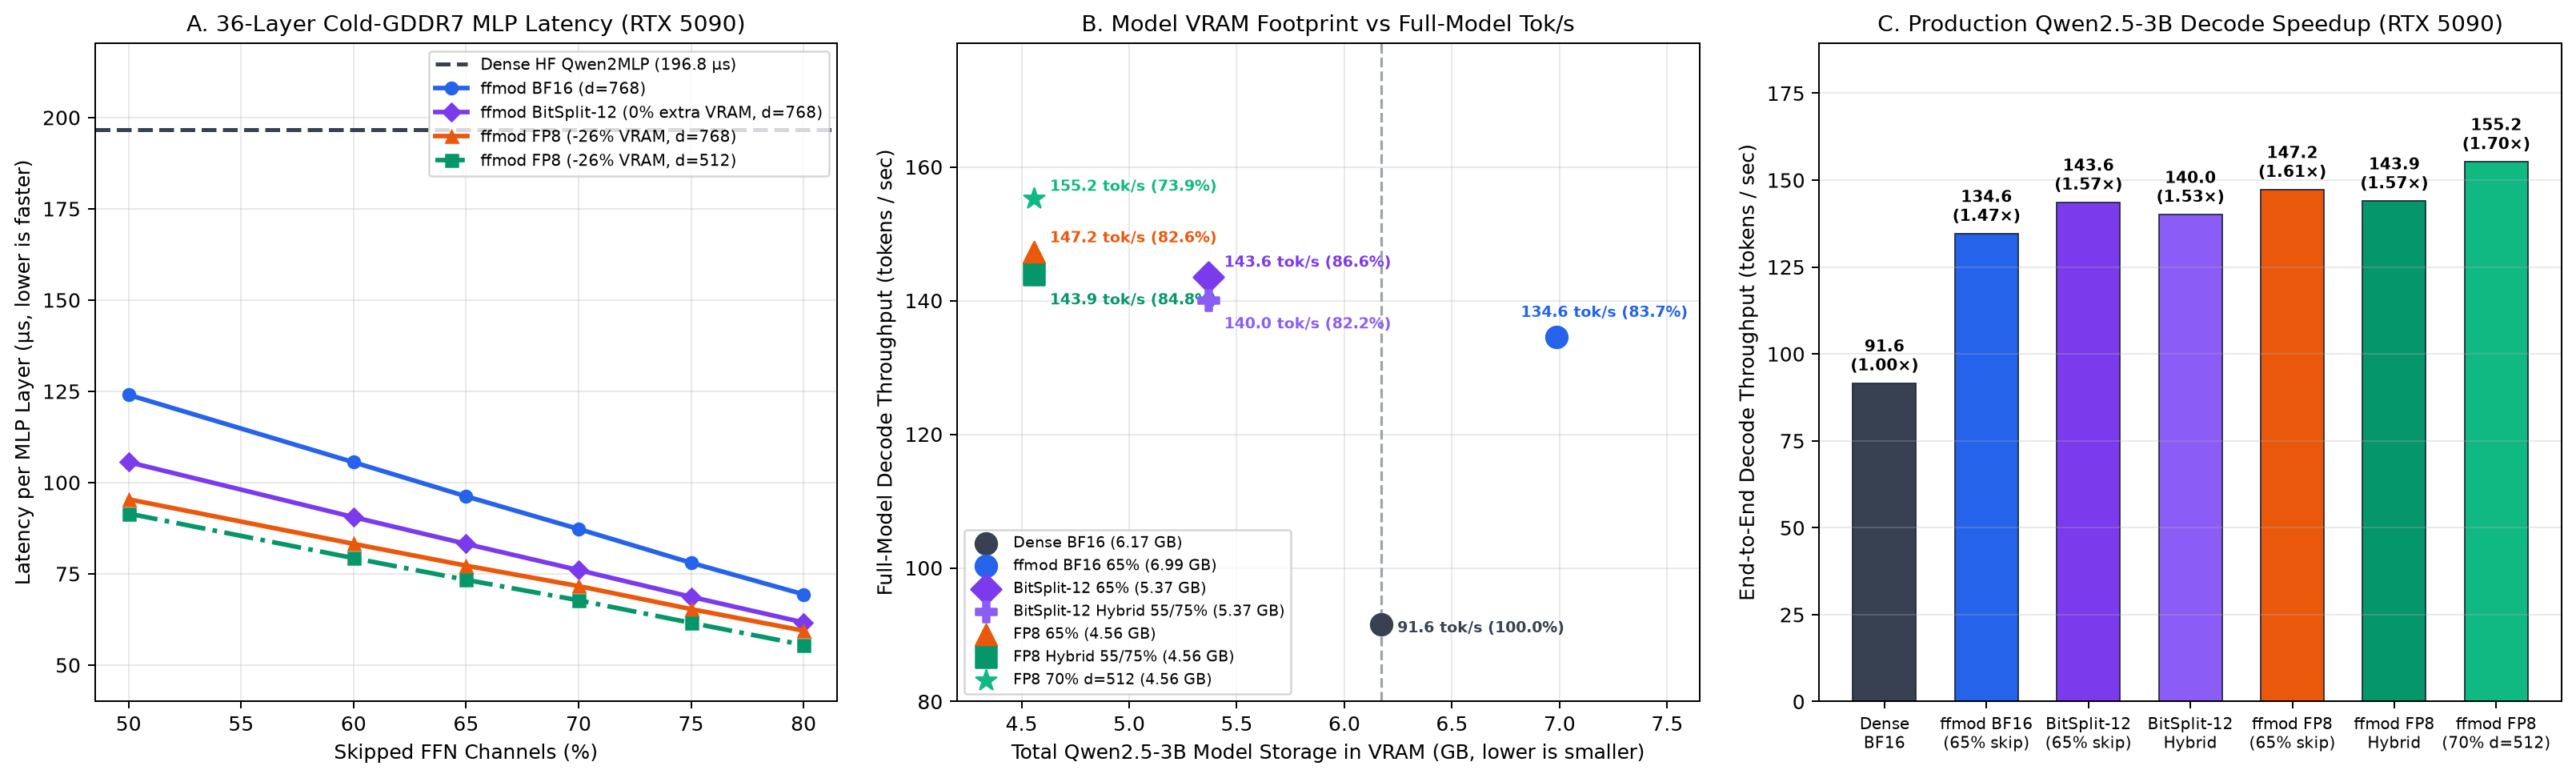
\includegraphics[width=0.97\textwidth]{../results/plots/fig7_production_fp8_bitsplit.png}
  \caption{\textbf{Experiment 8:} Production \texttt{BitSplit-12} and \texttt{FP8} sparse kernels simultaneously reduce VRAM ($6.17\to 4.56\text{--}5.37$~GB) and accelerate both single-token ($N=1$) and speculative ($N=4$) execution.}
  \label{fig:exp8}
\end{figure*}

Table~\ref{tab:exp8} and Fig.~\ref{fig:exp8} summarize cold-cache measurements across all 36 layers. Notably, at $N=4$ tokens (where dense \texttt{cuBLAS} shifts from GEMV to Tensor Cores at $186.5\,\mu$s), FFMod's union-active register broadcast reads each selected channel once and evaluates all 4 tokens in registers, achieving \textbf{$123.4\,\mu$s ($1.51\times$ faster than Tensor Cores!)} in \texttt{BitSplit-12}. End-to-end \texttt{Qwen2.5-3B} decoding accelerates from $91.6$~tok/s to \textbf{$143.6\text{--}155.2$~tok/s} ($1.57\times\text{--}1.70\times$), and sustains $131.2$~tok/s over live TCP HTTP/SSE streaming via \texttt{ffmod-serve}.

\section{Tiered GPU--DDR5 Execution over PCIe~5.0}
\label{sec:tiered}

Flagship $30\text{B}\text{--}70\text{B}+$ models exceed the $16\text{--}24$~GB VRAM of workstation and laptop GPUs even when quantized to 8-bit formats (e.g., \texttt{Qwen2.5-32B-Instruct} has $32.8\text{B}$ parameters: $65.5$~GB in \texttt{BF16} and $>33$~GB in \texttt{FP8}). However, its non-FFN parameters (embeddings, RMSNorms, GQA attention, LM head) plus all 64 layers' \texttt{Smooth-INT4} FFN indexes occupy only $\sim 13.7$~GB! Placing offloaded layers' $[I, 3, H]$ \texttt{FP8} channel payloads in page-locked (pinned) Host DDR5 RAM (\texttt{MADV\_HUGEPAGE} 2~MB Transparent Huge Pages) turns PCIe~5.0 x16 into a high-speed sparse channel bus.

\subsection{12-SM Open-Page DDR5 Coalesced UVA Gather}
When all 82 SMs of an RTX~5090 simultaneously issue Unified Virtual Addressing (UVA) reads to non-contiguous $15$~KB channels in host DDR5 RAM, concurrent requests hit dozens of distinct DRAM rows per channel/bank group, causing severe \textbf{DDR5 row-buffer bank thrashing} ($t_{\mathrm{RP}}+t_{\mathrm{RCD}}$ page-miss stalls) that caps throughput at $30.9$~GB/s while occupying $100\%$ of GPU SMs.

Restricting our coalesced \texttt{int64} gather kernel (\texttt{k\_uva\_gather\_fp8\_u64}) to \textbf{$12$~SMs} (\texttt{num\_warps=8}) keeps host DDR5 banks in sequential open-page burst mode, \textbf{increasing random channel gather bandwidth by $+22\text{--}28\%$ to $37.7\text{--}38.5$~GB/s} ($76\%$ of the $49.7\text{--}50.6$~GB/s contiguous \texttt{cudaMemcpyAsync} ceiling) while leaving \textbf{$70/82$ SMs ($85.4\%$ of the GPU)} completely free! Measured on concurrent priority CUDA streams (\texttt{s\_dma} + \texttt{s\_comp}), GPU compute overlaps with PCIe~5.0 gather at \textbf{$96.3\%\text{--}99.2\%$ hardware efficiency}.

\subsection{Core-Prefetch + Overlapped Exact Delta Fixup in \texttt{CUDAGraph}}
To hide PCIe transfer latency without sacrificing post-attention accuracy, FFMod installs PyTorch pre-hooks ahead of Self-Attention (and across preceding GPU-resident FFN layers when interleaved):
\begin{itemize}
  \item \textbf{\texttt{pre\_attn} (Speculative Fast Mode):} Predicts $K$ channels from the pre-attention state, streams them asynchronously into a double-buffered GDDR7 staging pool during Attention, and evaluates Stage~2 from $800$~GB/s GDDR7.
  \item \textbf{\texttt{pre\_attn\_exact\_delta} (Lossless-Channel Hybrid Mode):} Naive prefetching of all $K$ channels wastes $\sim 25\text{--}30\%$ PCIe bandwidth on borderline channels altered by Attention. Instead, FFMod prefetches only the \textbf{high-confidence core} $K_{\mathrm{pre}} = \lfloor 0.35 K\rfloor$ before Attention (where pre-attention precision exceeds $90\%$, incurring $<2.5\%$ wasted PCIe traffic!). After Attention finishes, exact post-attention Stage~1 routing and an O(1) L2 slot-table set-difference kernel (\texttt{k\_diff\_pre\_post\_channels}) execute on \texttt{comp\_stream} \emph{concurrently with the ongoing PCIe DMA}. Finally, \texttt{k4\_hybrid\_hit\_miss\_fp8} evaluates prefetched hits at $800$~GB/s from GDDR7 across all SMs while 12 SMs stream only the residual $S_{\mathrm{post}}\setminus S_{\mathrm{pre}}$ channels via UVA. Crucially, the entire 64-layer two-stream fork-join DAG is captured inside a single \textbf{\texttt{torch.cuda.CUDAGraph}}!
\end{itemize}

\subsection{Experiment 9: 64-Layer \texttt{Qwen2.5-32B-Instruct} Evaluation}
We evaluate the tiered PCIe~5.0 engine on full 64-layer \texttt{Qwen2.5-32B-Instruct} ($32.8\text{B}$ parameters, $H=5120, I=27648$, $65.53$~GB in \texttt{BF16}, $2.73\times$ larger than 24~GB VRAM) across two strict hardware profiles (Table~\ref{tab:exp9}, Fig.~\ref{fig:exp9}):
\begin{enumerate}
  \item \textbf{24~GB GPU Profile ($21.12$~GB VRAM + $26.33$~GB Pinned DDR5):} Keeps embeddings, GQA attention, LM head, all 64 \texttt{Smooth-INT4} indexes ($9.10$~GB), and 2 interleaved \texttt{FP8} FFN layers (layers~0 and 32) in GDDR7 while streaming 62 FFN layers over PCIe~5.0.
  \item \textbf{Strict 16~GB GPU Profile ($15.60$~GB VRAM + $31.85$~GB Pinned DDR5):} Compresses VRAM footprint by \textbf{$4.20\times$} vs.\ dense \texttt{BF16} by offloading all $64/64$ FFN layers plus $33/64$ \texttt{Smooth-INT4} indexes to UVA-mapped pinned DDR5!
\end{enumerate}

\begin{figure*}[t]
  \centering
  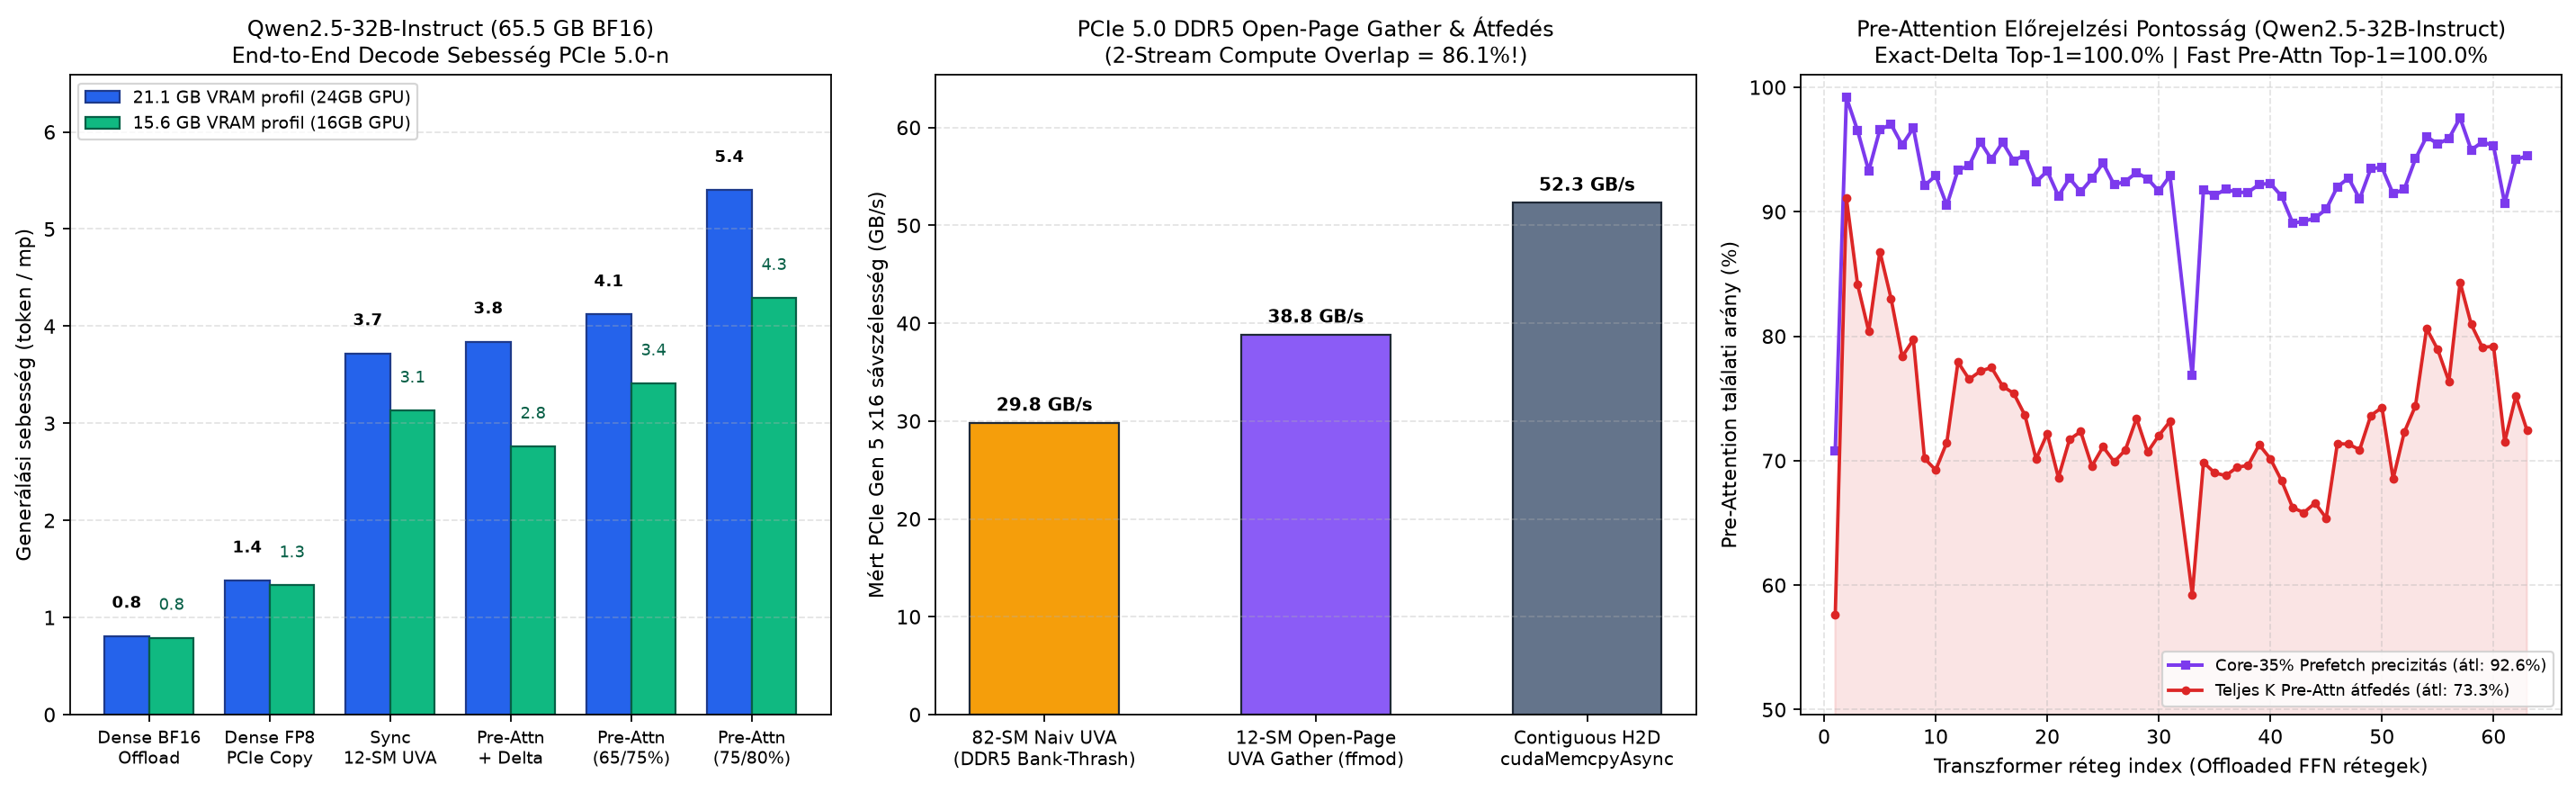
\includegraphics[width=0.98\textwidth]{../results/plots/fig8_pcie5_tiered_32b.png}
  \caption{\textbf{Experiment 9:} Full 64-layer \texttt{Qwen2.5-32B-Instruct} ($65.5$~GB \texttt{BF16}) tiered GPU--DDR5 execution over PCIe~5.0 x16 across $21.1$~GB and $15.6$~GB VRAM budgets, 12-SM open-page DDR5 gather physics ($38.8$~GB/s, $+30.2\%$ over 82-SM UVA), and layer-wise pre-attention core precision ($92.6\%$ mean) vs.\ full-$K$ overlap ($73.3\%$ mean).}
  \label{fig:exp9}
\end{figure*}

\begin{table*}[t]
  \centering
  \caption{End-to-end 64-layer \texttt{Qwen2.5-32B-Instruct} ($65.53$~GB \texttt{BF16}) PCIe~5.0 decode throughput, PCIe traffic per token, and held-out logit fidelity vs.\ full dense \texttt{FP8} reference across $21.12$~GB (24~GB GPU) and $15.60$~GB (16~GB GPU) VRAM profiles.}
  \label{tab:exp9}
  \resizebox{0.97\textwidth}{!}{%
  \begin{tabular}{lccccccc}
    \toprule
    \textbf{Offload Mode (\texttt{Qwen2.5-32B-Instruct})} & \textbf{PCIe~5.0} & \textbf{KL vs.} & \textbf{Top-1} & \multicolumn{2}{c}{\textbf{24~GB Profile ($21.12$~GB VRAM)}} & \multicolumn{2}{c}{\textbf{16~GB Profile ($15.60$~GB VRAM)}} \\
    \cmidrule(lr){5-6}\cmidrule(lr){7-8}
     & \textbf{Traffic/tok} & \textbf{Dense FP8} & \textbf{Match} & \textbf{Decode (tok/s)} & \textbf{Speedup} & \textbf{Decode (tok/s)} & \textbf{Speedup} \\
    \midrule
    Dense \texttt{BF16} PCIe Offload Baseline & $52.7\text{--}54.4$~GB & --- & $100\%$ & $0.81$~tok/s ($1229$~ms) & $1.00\times$ & $0.79$~tok/s ($1272$~ms) & $1.00\times$ \\
    Dense \texttt{FP8} Chunked PCIe Copy & $26.3\text{--}27.2$~GB & $0.0000$ & $100\%$ & $1.38$~tok/s ($726$~ms) & $1.70\times$ & $1.33$~tok/s ($752$~ms) & $1.68\times$ \\
    FFMod \texttt{sync\_uva} ($65/75\%$ skip, 12-SM) & $8.28\text{--}8.58$~GB & $0.0320$ & \textbf{$100.0\%$} & $3.72$~tok/s ($269$~ms) & $4.59\times$ & $3.13$~tok/s ($319$~ms) & $3.96\times$ \\
    \textbf{FFMod \texttt{pre\_attn\_exact\_delta}} ($65/75\%$) & $8.49\text{--}8.79$~GB & \textbf{$0.0139$} & \textbf{$100.0\%$} & \textbf{$3.84$~tok/s ($260$~ms)} & \textbf{$4.74\times$} & $2.76$~tok/s ($362$~ms) & $3.49\times$ \\
    \textbf{FFMod \texttt{pre\_attn}} ($65/75\%$ skip, \texttt{CUDAGraph}) & $8.28\text{--}8.58$~GB & \textbf{$0.0168$} & \textbf{$100.0\%$} & \textbf{$4.12$~tok/s ($243$~ms)} & \textbf{$5.09\times$} & \textbf{$3.41$~tok/s ($293$~ms)} & \textbf{$4.32\times$} \\
    \textbf{FFMod \texttt{pre\_attn}} ($75/80\%$ skip, \texttt{CUDAGraph}) & \textbf{$6.12\text{--}6.33$~GB} & \textbf{$0.0424$} & \textbf{$100.0\%$} & \textbf{$5.40$~tok/s ($185$~ms)} & \textbf{$6.67\times$} & \textbf{$4.29$~tok/s ($233$~ms)} & \textbf{$5.43\times$} \\
    \bottomrule
  \end{tabular}%
  }
\end{table*}

\textbf{Key Findings on 32B Scale:}
(1)~\emph{Superior Large-Model Sparsity Resilience:} Across all 32 multi-domain teacher-forced evaluation steps, every FFMod mode achieves \textbf{$100.0\%$ Top-1 agreement} with the full dense \texttt{FP8} model and remarkably low KL divergence ($\mathrm{KL}=0.0139$ in \texttt{pre\_attn\_exact\_delta}, $\mathrm{KL}=0.0168$ in \texttt{pre\_attn} $65/75\%$, and $\mathrm{KL}=0.0424$ even at $75/80\%$ skip).
(2)~\emph{92.6\% Core Prefetch Precision:} Across the 60 intra-block pre-attention layers, our $\lfloor 0.35 K\rfloor$ core achieves $90.5\%\text{--}99.2\%$ hit precision ($92.64\%$ overall mean; $73.34\%$ full-$K$ overlap), while layers~1 and 33---which look ahead across \emph{both} a preceding GPU FFN and Self-Attention---still retain $70.8\%\text{--}76.9\%$ core precision.
(3)~\emph{$4.74\times\text{--}6.67\times$ Wall-Clock Speedup:} Under the 24~GB profile, \texttt{pre\_attn\_exact\_delta} ($3.84$~tok/s) outperforms synchronous UVA ($3.72$~tok/s) with lossless channel parity, while speculative \texttt{pre\_attn} reaches \textbf{$4.12\text{--}5.40$~tok/s ($5.09\times\text{--}6.67\times$ over dense \texttt{BF16} offload)}, cutting PCIe traffic by $88.4\%$ ($52.7 \to 6.12$~GB/token). Under the $15.60$~GB cap (where 33 INT4 indexes also reside on host UVA, penalizing dual-scan \texttt{exact\_delta}), single-scan \texttt{pre\_attn} sustains \textbf{$3.41\text{--}4.29$~tok/s ($4.32\times\text{--}5.43\times$)}.
(4)~\emph{VRAM-First Auto Placement \& Budget-Independent Sharded Cache:} FFMod unifies pure in-VRAM and tiered execution behind an automatic VRAM-first allocator (\texttt{--tiered-vram-gb auto}) that places $100\%$ of layers in GDDR7 with zero host RAM usage whenever a model fits, spilling only excess layers to pinned DDR5. Moreover, because the canonical per-layer tuple (\texttt{w\_idx\_i32}, \texttt{w\_ch\_fp8}, scales) is invariant to runtime sparsity and VRAM placement, FFMod persists 64 atomic \texttt{safetensors} shards (\texttt{.ffmod\_cache\_v1}, $36.28$~GB vs.\ $65.54$~GB \texttt{BF16}, $1.81\times$ smaller on disk) using $<1.5$~GB peak VRAM, hydrating any GPU/DDR5 budget split bit-identically at $0.169$~s/layer ($\sim 10.8$~s for 64 layers on PCIe NVMe) with zero re-quantization.

\section{Related Work}
\label{sec:related}

Table~\ref{tab:related} contrasts FFMod against representative sparse inference frameworks. Learned-predictor systems (\textbf{DejaVu}~\cite{liu2023dejavu}, \textbf{PowerInfer}~\cite{song2024powerinfer}, \textbf{LLM in a Flash}~\cite{alizadeh2024llmflash}) achieve strong speedups on ReLU models~\cite{mirzadeh2024relustrikesback} but require model conversion or per-layer predictor training and add VRAM overhead. Among training-free SwiGLU methods, \textbf{CATS}~\cite{lee2024cats} evaluates $100\%$ of $W_{\mathrm{gate}}$ in 16-bit precision and relies on calibrated thresholds; \textbf{TEAL}~\cite{liu2025teal} and \textbf{R-Sparse}~\cite{zhang2025rsparse} prune input coordinates or low-rank SVD components inside the main projection, limiting practical sparsity to $40\text{--}50\%$; \textbf{CoreInfer}~\cite{wang2025coreinfer} freezes sentence-level neurons at prefill, missing token-level reasoning spikes; and \textbf{Double Sparsity}~\cite{yang2024doublesparsity} targets KV-cache attention tokens rather than gated FFN channels. FFMod uniquely unifies zero-data dual-branch \texttt{Smooth-INT4} routing ($\sim 4.7\%$ traffic), exact full-$H$ evaluation, negative-VRAM \texttt{BitSplit-12}/\texttt{FP8} storage, and two-stream \texttt{CUDAGraph} PCIe~5.0 core-delta prefetching.

\begin{table*}[t]
  \centering
  \caption{Architectural comparison of FFMod against prior sparse LLM inference frameworks.}
  \label{tab:related}
  \resizebox{0.96\textwidth}{!}{%
  \begin{tabular}{lccccc}
    \toprule
    \textbf{System} & \textbf{Native SwiGLU?} & \textbf{Zero Data \& Zero Train?} & \textbf{Router Traffic} & \textbf{Net VRAM vs.\ BF16} & \textbf{PCIe~5.0 Prefetch + Exact Delta?} \\
    \midrule
    PowerInfer~\cite{song2024powerinfer} & No (ReLU conversion) & No (Trained MLP) & $\sim 5\%$ & $+15\%$ to $+20\%$ & Reactive / CPU hybrid \\
    CATS~\cite{lee2024cats} & Yes & Calibrated thresholds & $33.3\%$ ($100\%$ of $W_{\mathrm{gate}}$) & $0\%$ & No \\
    TEAL~\cite{liu2025teal} & Yes & Calibrated histograms & Input coordinate crop & $0\%$ & No \\
    CoreInfer~\cite{wang2025coreinfer} & Yes & Yes & Static sentence prefill & $0\%$ & No \\
    \textbf{FFMod (Ours)} & \textbf{Yes (+GeGLU)} & \textbf{100\% Zero-Data} & \textbf{$4.2\%\text{--}6.3\%$ (\texttt{Smooth-INT4})} & \textbf{$-13.0\%$ to $-26.1\%$} & \textbf{Yes (2-Stream \texttt{CUDAGraph})} \\
    \bottomrule
  \end{tabular}%
  }
\end{table*}

\section{Conclusion}
Separating parameter storage from dynamic compute planning unlocks substantial headroom on modern GPUs without touching pretrained weights. By indexing gated FFN layers via zero-data \texttt{Smooth-INT4 $\times$ Top-$D$} scans, pairing them with \texttt{BitSplit-12} and \texttt{FP8} channel payloads, respecting KV-cache error dynamics across depth, and co-designing a 12-SM open-page DDR5 gather pipeline over PCIe~5.0, FFMod delivers $1.57\times\text{--}1.70\times$ faster in-VRAM generation in $26\%$ less memory and makes $32\text{B}+$ models fast and practical on single $16\text{--}24$~GB GPUs.

\bibliographystyle{plain}
\bibliography{references}

\end{document}
